\section{Super-Admin}

Di seguito vengono elencati i \glossaryItem{casi} d'uso per il \glossaryItem{Super-Admin}.

%''Fig. 29 e seguenti: esistono \glossaryItem{casi} d’uso senza codice identificativo.
%Questi non hanno alcuna descrizione associata. Tutti i \glossaryItem{diagrammi} dei \glossaryItem{casi}
%d’uso devono avere associata una relativa descrizione (come fatto fino a
%questo punto).''

\subsection{Casi d'uso}

\subsubsection{Interazione ad alto livello tra sistema e super-admin}

    \begin{figure}[h]
      \begin{center}
        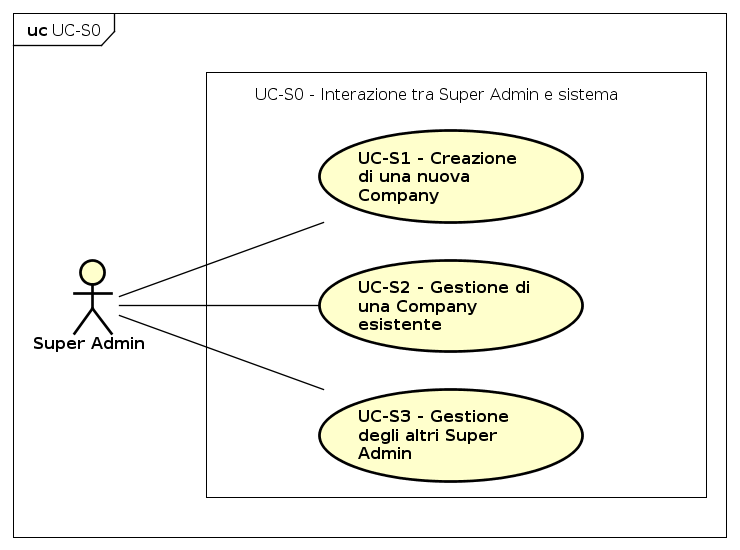
\includegraphics[width=12cm]{res/img/UCSuperadmin/UC-S0.png}
      \caption{UC-S0 - Interazione tra \glossaryItem{Super-Admin} e sistema}
      \end{center} 
    \end{figure}    
    
    %Tabella 
    \begin{center}
      \bgroup
      \def\arraystretch{1.8}     
      \begin{longtable}{  p{3.5cm} | p{8cm} } 
        
        \hline
        \multicolumn{2}{ | c | }{ \cellcolor[gray]{0.9} \textbf{UC-S0 - Gestione \glossaryItem{Company}}} \\ 
        \hline
        
        \textbf{Attori Primari} & \glossaryItem{Super-Admin}.\\ 
	\textbf{Scopo e descrizione} & Il \glossaryItem{Super-Admin} deve poter gestire i dati dell'applicazione \glossaryItem{MaaS}.  \\ 
        \textbf{Precondizioni}  & L'applicazione mostra al \glossaryItem{Super-Admin} la pagina di gestione di \glossaryItem{MaaS}.  \\ 
        
        \textbf{Postcondizioni} & L'applicazione ha dato la possibilità al \glossaryItem{Super-Admin} di gestire \glossaryItem{MaaS}. \\ 
        \textbf{Scenario principale} & 1. Il \glossaryItem{Super-Admin} pu\`o creare una nuova \glossaryItem{Company}. (UC-S1) 
        
        2. Il \glossaryItem{Super-Admin} può gestire in dettaglio una \glossaryItem{Company} esistente. (UC-S2)
        
        3. Il \glossaryItem{Super-Admin} può gestire gli altri \glossaryItem{Super-Admin} dell'applicazione. (UC-S3)  \\ 
        
      \end{longtable}
      \egroup
    \end{center}

\subsubsection{Creazione di una nuova Company}
    \begin{figure}[H]
      \begin{center}
        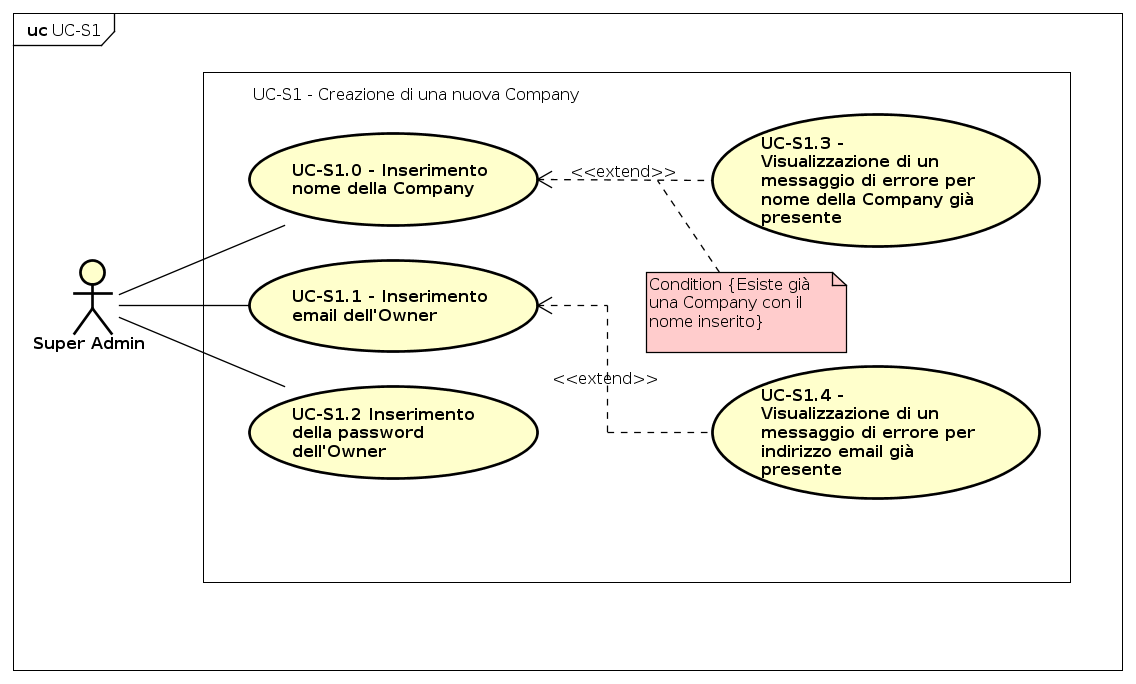
\includegraphics[width=12cm]{res/img/UCSuperadmin/UC-S1.png}
      \caption{UC-S1 - Creazione di una nuova \glossaryItem{Company}}
      \end{center} 
    \end{figure}    
    
    %Tabella 
    \begin{center}
      \bgroup
      \def\arraystretch{1.8}     
      \begin{longtable}{  p{3.5cm} | p{8cm} } 
        
        \hline
        \multicolumn{2}{ | c | }{ \cellcolor[gray]{0.9} \textbf{UC-S1 - Creazione di una nuova \glossaryItem{Company}}} \\ 
        \hline
        
        \textbf{Attori Primari} & \glossaryItem{Super-Admin}.\\  
        \textbf{Scopo e descrizione} & L'applicazione offre un form nel quale il \glossaryItem{Super-Admin} può inserire i dati necessari alla creazione di una nuova \glossaryItem{Company} \\
        \textbf{Precondizioni}  & Il sistema fornisce al \glossaryItem{Super-Admin} un form di registrazione.  \\ 
        
        \textbf{Postcondizioni} & Il sistema ha aggiunto una nuova \glossaryItem{Company} e il suo \glossaryItem{Owner}. \\ 
        \textbf{Scenario principale} & 1. Il \glossaryItem{Super-Admin} inserisce il nome della \glossaryItem{Company}. (UC-S1.0)
        
        2. Il \glossaryItem{Super-Admin} inserisce la propria email. (UC-S1.1)
        
        3. Il \glossaryItem{Super-Admin} inserisce una password. (UC-S1.2) \\ 
        \textbf{Estensioni} & 1. la \glossaryItem{Company} esiste gi\`a. (UC-S1.3)
        
        2. L'email inserita \`e gi\`a stata usata. (UC-S1.4) \\
      \end{longtable}
      \egroup
    \end{center}

%%DA FARE
    \subsubsection{Creazione di una nuova Company - Inserimento del nome della nuova Company}
    
    %Tabella 
    \begin{center}
          \bgroup
          \def\arraystretch{1.8}     
          \begin{longtable}{  p{3.5cm} | p{8cm} } 
            
            \hline
            \multicolumn{2}{ | c | }{ \cellcolor[gray]{0.9} \textbf{UC-S1.0 - Inserimento del nome della \glossaryItem{Company} }} \\ 
        \hline
        
        \textbf{Attori Primari} & \glossaryItem{Super-Admin}\\  
        \textbf{Scopo e descrizione} & L'applicazione offre un campo testo su cui il \glossaryItem{Super-Admin} può scrivere il nome della \glossaryItem{Company} \\
      
        \textbf{Precondizioni}  & L'applicazione offre un campo testo. \\ 
        
        \textbf{Postcondizioni} & Il \glossaryItem{Super-Admin} ha compilato il campo testo relativo al nome della \glossaryItem{Company} \\ 
        
        \textbf{Scenario principale} & 1. Il \glossaryItem{Super-Admin} inserisce il nome della \glossaryItem{Company} nel \textit{form} offerto dall'applicazione. \\
        
        \textbf{Estensioni} & 1. Il nome della \glossaryItem{Company} inserito è già presente in \glossaryItem{MaaS}. (UC-S1.3)
     \end{longtable}
      \egroup
    \end{center}



\subsubsection{Creazione di una nuova Company - Inserimento dell'email dell'Owner della nuova Company}
    
    %Tabella 
    \begin{center}
          \bgroup
          \def\arraystretch{1.8}     
          \begin{longtable}{  p{3.5cm} | p{8cm} } 
            
            \hline
            \multicolumn{2}{ | c | }{ \cellcolor[gray]{0.9} \textbf{UC-S1.1 - Inserimento della email dell'\glossaryItem{Owner} }} \\ 
        \hline
        
        \textbf{Attori Primari} & \glossaryItem{Super-Admin}\\  
        \textbf{Scopo e descrizione} & Il \glossaryItem{Super-Admin} può inserire l'indirizzo email dell'\glossaryItem{Owner} nel campo del form offerto dall'applicazione \\
      
        \textbf{Precondizioni}  & L'applicazione offre un campo testo. \\ 
        
        \textbf{Postcondizioni} & Il \glossaryItem{Super-Admin} ha compilato il campo testo relativo all'email dell'\glossaryItem{Owner} \\ 
        
        \textbf{Scenario principale} & 1. Il \glossaryItem{Super-Admin} inserisce l'indirizzo email dell'Owner nel \textit{form} offerto dall'applicazione. \\
        
        \textbf{Estensioni} & 1. L'indirizzo email inserito è già presente in \glossaryItem{MaaS}. (UC-S1.4)
     \end{longtable}
      \egroup
    \end{center}

    \subsubsection{Creazione di una nuova Company - Inserimento della password dell'Owner} 
    
    %Tabella 
    \begin{center}
      \bgroup
      \def\arraystretch{1.8}     
      \begin{longtable}{  p{3.5cm} | p{8cm} } 
        
        \hline
        \multicolumn{2}{ | c | }{ \cellcolor[gray]{0.9} \textbf{UC-S1.2 - Inserimento della password dell'\glossaryItem{Owner} }} \\ 
        \hline
        
        \textbf{Attori Primari} & \glossaryItem{Super-Admin}\\  
        \textbf{Scopo e descrizione} & L'applicazione offre un campo testo offuscato su cui il \glossaryItem{Super-Admin} può scrivere la password dell'\glossaryItem{Owner} \\
      
        \textbf{Precondizioni}  & L'applicazione mostra un campo testo offuscato. \\ 
        
        \textbf{Postcondizioni} & Il \glossaryItem{Super-Admin} ha compilato il campo testo relativo alla password dell'\glossaryItem{Owner} \\ 
        \\
        \textbf{Scenario principale} & 1. Il \glossaryItem{Super-Admin} inserisce la password dell'Owner nel \textit{form} offerto dall'applicazione.
     \end{longtable}
      \egroup
    \end{center}

\subsubsection{Fallimento della creazione di una Company - Nome della Company già presente} 
    
    %Tabella 
    \begin{center}
      \bgroup
      \def\arraystretch{1.8}     
      \begin{longtable}{  p{3.5cm} | p{8cm} } 
        
        \hline
        \multicolumn{2}{ | c | }{ \cellcolor[gray]{0.9} \textbf{UC-S1.3 - Il nome della \glossaryItem{Company} è già presente}} \\ 
        \hline
        
        \textbf{Attori Primari} & \glossaryItem{Super-Admin}\\  
        \textbf{Scopo e descrizione} & Il \glossaryItem{Super-Admin} ha inserito un nome della \glossaryItem{Company} già presente nell'applicazione e il sistema comunica l'errore. \\
      
        \textbf{Precondizioni}  & L'applicazione ha ricevuto in input dei dati non validi per la creazione di una \glossaryItem{Company}. \\ 
        
        \textbf{Postcondizioni} & Il sistema mostra al \glossaryItem{Super-Admin} un messaggio di errore che comunica l'entità dell'input errato. \\ 
         \textbf{Scenario principale} & 1. Il \glossaryItem{Super-Admin} visualizza l'errore. \\
        
     \end{longtable}
      \egroup
    \end{center}

\subsubsection{Fallimento della creazione di una Company - Indirizzo email dell'Owner già presente} 
    
    %Tabella 
    \begin{center}
      \bgroup
      \def\arraystretch{1.8}     
      \begin{longtable}{  p{3.5cm} | p{8cm} } 
        
        \hline
        \multicolumn{2}{ | c | }{ \cellcolor[gray]{0.9} \textbf{UC-S1.4 - L'indirizzo email dell'Owner è già presente}} \\ 
        \hline
        
        \textbf{Attori Primari} & \glossaryItem{Super-Admin}\\  
        \textbf{Scopo e descrizione} & Il \glossaryItem{Super-Admin} ha inserito un indirizzo email già presente nell'applicazione e il sistema comunica l'errore. \\
      
        \textbf{Precondizioni}  & Il sistema ha ricevuto in input dei dati non validi per la creazione di una \glossaryItem{Company}. \\ 
        
        \textbf{Postcondizioni} & Il sistema mostra al \glossaryItem{Super-Admin} un messaggio di errore che comunica l'entità dell'input errato. \\ 
         \textbf{Scenario principale} & 1. Il \glossaryItem{Super-Admin} visualizza l'errore. \\
        
     \end{longtable}
      \egroup
    \end{center}



    \subsubsection{Gestione in dettaglio di una Company esistente}
    \begin{figure}[H]
      \begin{center}
        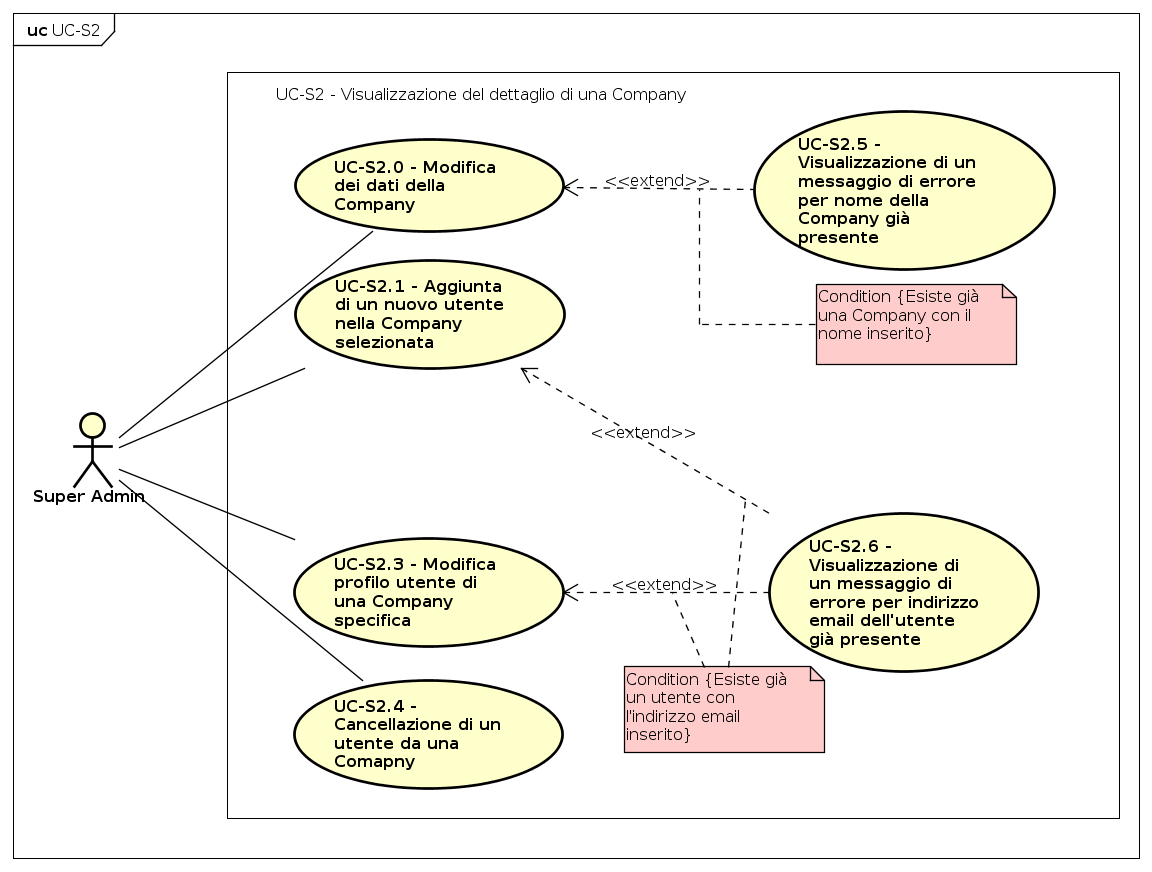
\includegraphics[width=12cm]{res/img/UCSuperadmin/UC-S2.png}
      \caption{UC-S2 - Gestione in dettaglio di una \glossaryItem{Company} esistente}
      \end{center} 
    \end{figure}    
    
    %Tabella 
    \begin{center}
      \bgroup
      \def\arraystretch{1.8}     
      \begin{longtable}{  p{3.5cm} | p{8cm} } 
        
        \hline
        \multicolumn{2}{ | c | }{ \cellcolor[gray]{0.9} \textbf{UC-S2 - Gestione in dettaglio di una \glossaryItem{Company} esistente}} \\ 
        \hline
        
        \textbf{Attori Primari} & \glossaryItem{Super-Admin}\\  
        \textbf{Scopo e descrizione} & Il \glossaryItem{Super-Admin} visualizza una pagina contenente i dettagli di una \glossaryItem{Company} e può apportare delle modifiche alla \glossaryItem{Company} o ai suoi utenti. \\
        \textbf{Precondizioni}  & L'applicazione mette a disposizione la pagina di gestione di una \glossaryItem{Company}.  \\ 
        
        \textbf{Postcondizioni} & L'applicazione ha effettuato le operazioni richeste dal \glossaryItem{Super-Admin}. \\
        
        \textbf{Scenario principale} & 1. Il \glossaryItem{Super-Admin} può modificare i dati della \glossaryItem{Company} (UC-S2.0);  
        
        2. Il \glossaryItem{Super-Admin} può aggiungere un nuovo utente della \glossaryItem{Company} (UC-S2.1);
        
        3. Il \glossaryItem{Super-Admin} può visualizzare uno specifico utente della \glossaryItem{Company} (UC-S2.2); 
        
        4. Il \glossaryItem{Super-Admin} pu\`o modificare i dati di uno specifico utente (UC-S2.3);
        
        5. Il \glossaryItem{Super-Admin} pu\`o cancellare uno specifico utente. (UC-S2.4) \\ 
        
        \textbf{Estensioni} & 1. Fallimento della modifica dei dati della \glossaryItem{Company} (UC-S2.5);
        
        2. Fallimento dell'aggiunta di un nuovo utente (UC-S2.6);
        
        3. Fallimento modifica utente (UC-S2.6). \\
      \end{longtable}
      \egroup
    \end{center}


\subsubsection{Modifica dei dati di una Company}
    \begin{figure}[H]
      \begin{center}
        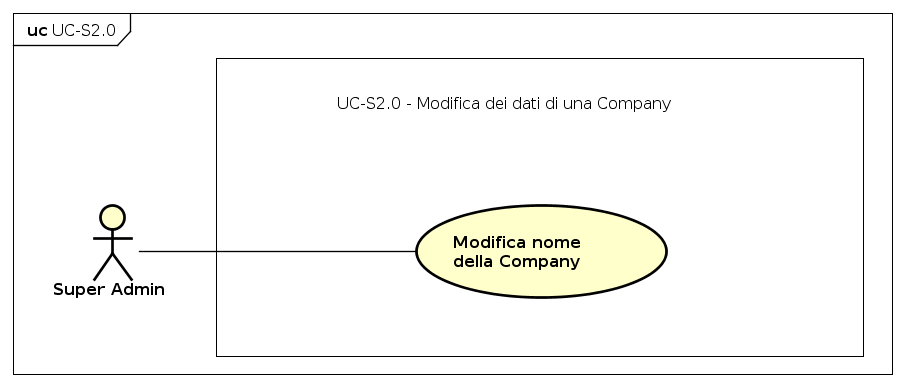
\includegraphics[width=12cm]{res/img/UCSuperadmin/UC-S2.0.png}
      \caption{UC-S2.0 - Modifica dei dati di una \glossaryItem{Company}}
      \end{center} 
    \end{figure}    
    
    %Tabella 
    \begin{center}
      \bgroup
      \def\arraystretch{1.8}     
      \begin{longtable}{  p{3.5cm} | p{8cm} } 
        
        \hline
        \multicolumn{2}{ | c | }{ \cellcolor[gray]{0.9} \textbf{UC-S2.0 - Modifica dei dati di una \glossaryItem{Company}}}. \\ 
        \hline
        
        \textbf{Attori Primari} & \glossaryItem{Super-Admin}.\\  
        \textbf{Scopo e descrizione} & Il \glossaryItem{Super-Admin} visualizza una \textit{form} per la modifica dei dati di una \glossaryItem{Company}. \\
        \textbf{Precondizioni}  & L'applicazione mostra il form per la modifica dei dati della \glossaryItem{Company} selezionata.  \\ 
        
        \textbf{Postcondizioni} & Il sistema ha modificato il profilo della \glossaryItem{Company} sulla base dei dati inseriti dal \glossaryItem{Super-Admin}.  \\ 
       	 \textbf{Scenario principale} & 1. Il \glossaryItem{Super-Admin} può modificare il nome della \glossaryItem{Company} (UC-S2.0.0). \\
	 \textbf{Estensioni} & 1. Fallimento della modifica (UC-S2.5).
      \end{longtable}
      \egroup
    \end{center}

%INTERNO: 2.0.0 --> PUBBLICATO
\subsubsection{Modifica del nome di una Company}
    %Tabella 
    \begin{center}
      \bgroup
      \def\arraystretch{1.8}
      \begin{longtable}{  p{3.5cm} | p{8cm} }

        \hline
        \multicolumn{2}{ | c | }{ \cellcolor[gray]{0.9} \textbf{UC-S2.0.0 - Modifica del nome di una \glossaryItem{Company}}}. \\
        \hline

        \textbf{Attori Primari} & \glossaryItem{Super-Admin}.\\
	\textbf{Scopo e descrizione}  & Il Super-Admin deve poter modificare il nome della \glossaryItem{Company}.  \\
        \textbf{Precondizioni}  & L'applicazione mostra il campo di testo per la modifica del nome della \glossaryItem{Company} selezionata.  \\
	
        \textbf{Postcondizioni} & Il sistema ha modificato il nome della \glossaryItem{Company} sulla base del nuovo nome inserito dal \glossaryItem{Super-Admin}.  \\
    	\textbf{Scenario principale} & 1. Il \glossaryItem{Super-Admin} può modificare il nome della \glossaryItem{Company}. \\
        \textbf{Estensioni} & 1. Fallimento della modifica (UC-S2.5).
      \end{longtable}
      \egroup
    \end{center}






\subsubsection{Aggiunta di un nuovo utente nella Company selezionata}
    \begin{figure}[H]
      \begin{center}
        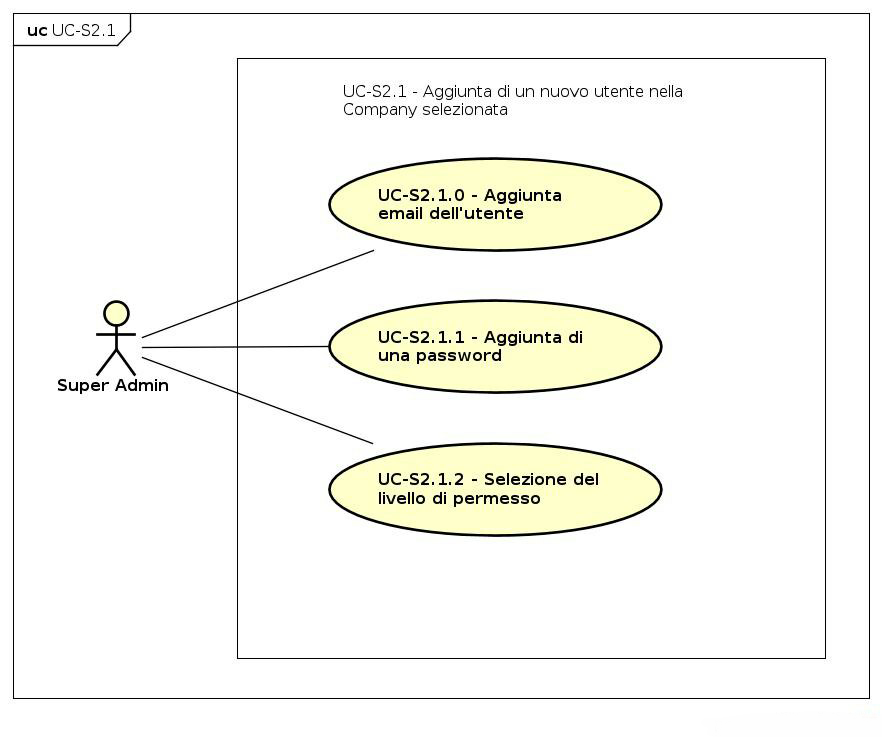
\includegraphics[width=12cm]{res/img/UCSuperadmin/UC-S2.1.png}
      \caption{UC-S2.1 - Aggiunta di un nuovo utente nella \glossaryItem{Company} selezionata}
      \end{center} 
    \end{figure}    
    
    %Tabella 
    \begin{center}
      \bgroup
      \def\arraystretch{1.8}     
      \begin{longtable}{  p{3.5cm} | p{8cm} } 
        
        \hline
        \multicolumn{2}{ | c | }{ \cellcolor[gray]{0.9} \textbf{UC-S2.1 - Aggiunta di un nuovo utente nella \glossaryItem{Company} selezionata}} \\ 
        \hline
        
        \textbf{Attori Primari} & \glossaryItem{Super-Admin}.\\ 
      	\textbf{Scopo e descrizione}  & Il Super-Admin aggiunge un nuovo utente alla \glossaryItem{Company} selezionata.  \\ 
        \textbf{Precondizioni}  & L'applicazione mostra il form per l'aggiunta di un nuovo utente.  \\ 
        
        \textbf{Postcondizioni} & Il sistema ha aggiunto un nuovo utente associandolo alla \glossaryItem{Company} selezionata.  \\ 
	\textbf{Scenario principale} & 1. Il \glossaryItem{Super-Admin} può aggiungere l'email dell'utente (UC-S2.1.0);

        2. Il \glossaryItem{Super-Admin} può aggiungere la password dell'utente (UC-S2.1.1);

        3. Il \glossaryItem{Super-Admin} può selezionare il livello di permesso dell'utente (UC-S2.1.2). \\

        \textbf{Estensioni} & 1. Fallimento dell'aggiunta di un nuovo utente (UC-S2.6).
 	


	 \end{longtable}
      \egroup
    \end{center}

%
\subsubsection{Aggiunta dell'email dell'utente}

    %Tabella 
    \begin{center}
      \bgroup
      \def\arraystretch{1.8}
      \begin{longtable}{  p{3.5cm} | p{8cm} }

        \hline
        \multicolumn{2}{ | c | }{ \cellcolor[gray]{0.9} \textbf{UC-S2.1.0 - Aggiunta dell'email dell'utente}} \\
        \hline

        \textbf{Attori Primari} & \glossaryItem{Super-Admin}.\\
        \textbf{Scopo e descrizione}  & Il Super-Admin inserisce l'indirizzo email del nuovo utente.  \\ 
        \textbf{Precondizioni}  & L'applicazione mostra il campo di testo per l'aggiunta dell'email del nuovo utente.  \\

        \textbf{Postcondizioni} & Il sistema ha memorizzato l'email inserita nel campo di testo.  \\
	\textbf{Scenario principale} & Il Super-Admin inserisce l'email dell'utente da aggiungere.  \\ 
      \end{longtable}
      \egroup
    \end{center}


\newpage

\subsubsection{Aggiunta della password dell'utente}

    %Tabella 
    \begin{center}
      \bgroup
      \def\arraystretch{1.8}
      \begin{longtable}{  p{3.5cm} | p{8cm} }

        \hline
        \multicolumn{2}{ | c | }{ \cellcolor[gray]{0.9} \textbf{UC-S2.1.1 - Aggiunta della password dell'utente}} \\
        \hline

        \textbf{Attori Primari} & \glossaryItem{Super-Admin}.\\
        \textbf{Scopo e descrizione}  & Il Super-Admin inserisce la password del nuovo utente.  \\ 
        \textbf{Precondizioni}  & L'applicazione mostra il campo di testo per l'aggiunta della password del nuovo utente.  \\

        \textbf{Postcondizioni} & Il sistema ha memorizzato la password inserita nel campo di testo.  \\
        \textbf{Scenario principale} & Il Super-Admin inserisce la password dell'utente da aggiungere.  \\
      \end{longtable}
      \egroup
    \end{center}


\subsubsection{Selezione del livello di permesso per l'utente}

    %Tabella 
    \begin{center}
      \bgroup
      \def\arraystretch{1.8}
      \begin{longtable}{  p{3.5cm} | p{8cm} }

        \hline
        \multicolumn{2}{ | c | }{ \cellcolor[gray]{0.9} \textbf{UC-S2.1.2 - Selezione del livello di permesso per l'utente}} \\
        \hline

        \textbf{Attori Primari} & \glossaryItem{Super-Admin}.\\
        \textbf{Scopo e descrizione}  & Il Super-Admin inserisce il livello di permesso del nuovo utente.  \\ 
        \textbf{Precondizioni}  & L'applicazione permette al Super-Admin di selezionare il livello di permesso per l'utente da aggiungere.  \\

        \textbf{Postcondizioni} & Il sistema ha memorizzato il livello di permesso selezionato.  \\
        \textbf{Scenario principale} & Il Super-Admin seleziona il livello di permesso dell'utente da aggiungere.  \\
      \end{longtable}
      \egroup
    \end{center}



\subsubsection{Visualizzazione in dettaglio di un utente della Company}
    %Tabella 
    \begin{center}
      \bgroup
      \def\arraystretch{1.8}     
      \begin{longtable}{  p{3.5cm} | p{8cm} } 
        
        \hline
        \multicolumn{2}{ | c | }{ \cellcolor[gray]{0.9} \textbf{UC-S2.2 - Visualizzazione in dettaglio di un utente della \glossaryItem{Company}}} \\ 
        \hline
        
        \textbf{Attori Primari} & \glossaryItem{Super-Admin}\\  
        \textbf{Scopo e descrizione} & Il \glossaryItem{Super-Admin} entra nella pagina di visualizzazione del profilo di un utente. \\
        \textbf{Precondizioni}  & Il sistema presenta la pagina di visualizzazione in dettaglio di un utente.  \\ 
        
        \textbf{Postcondizioni} & Il sistema ha ricevuto l'input dal \glossaryItem{Super-Admin}.  \\ 
         \textbf{Scenario principale} & 1. Il \glossaryItem{Super-Admin} visualizza il profilo dell'utente. \\
        
     
     \end{longtable}
      \egroup
    \end{center}

\subsubsection{Modifica del profilo di un utente}
    \begin{figure}[H]
      \begin{center}
        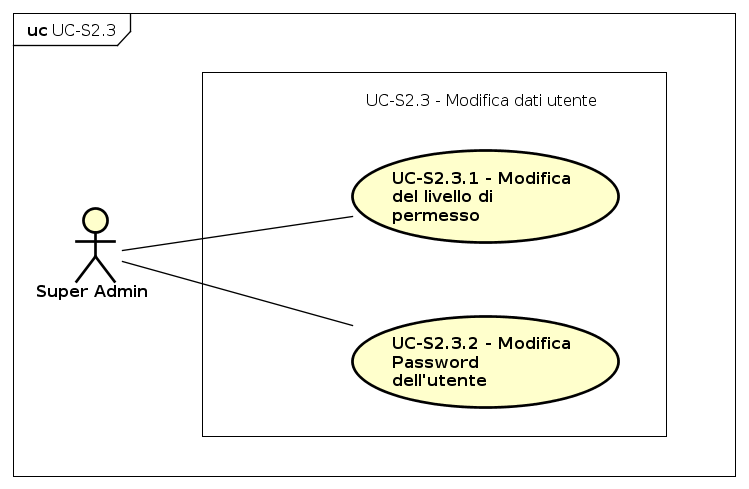
\includegraphics[width=12cm]{res/img/UCSuperadmin/UC-S2.3.png}
      \caption{UC-S2.3 - Modifica del profilo di un utente}
      \end{center} 
    \end{figure}    
    
    %Tabella 
    \begin{center}
      \bgroup
      \def\arraystretch{1.8}     
      \begin{longtable}{  p{3.5cm} | p{8cm} } 
        
        \hline
        \multicolumn{2}{ | c | }{ \cellcolor[gray]{0.9} \textbf{UC-S2.3 - Modifica del profilo di un utente }} \\ 
        \hline
        
        \textbf{Attori Primari} & \glossaryItem{Super-Admin}\\  
        \textbf{Scopo e descrizione} & Il \glossaryItem{Super-Admin} entra nella pagina di modifica dell'utente, nella quale ha la possibilit\`a
        di modificarne ruolo e password. \\
      
        \textbf{Precondizioni}  & L'applicazione offre un form di modifica del profilo. \\ 
        
        \textbf{Postcondizioni} & Il sistema ha modificato il profilo dell'utente sulla base di quanto inserito dal \glossaryItem{Super-Admin}. \\ 
         \textbf{Scenario principale} & 1. Il \glossaryItem{Super-Admin} ha la possibilit\`a di modificare la tipologia dell'utente. (UC-S2.3.1);
         
         2. Il \glossaryItem{Super-Admin} ha la possibilit\`a di modificare la password dell'utente. (UC-S2.3.2) \\
        
        
         \textbf{Estensioni} & 1. Fallimento della modifica dell'utente (UC-S2.6).  \\
     
     \end{longtable}
      \egroup
    \end{center}

%INTERNO: 2.3.1 "Modifica del livello di permesso""

\subsubsection{Modifica del livello di permesso}
    %Tabella 
    \begin{center}
      \bgroup
      \def\arraystretch{1.8}     
      \begin{longtable}{  p{3.5cm} | p{8cm} } 
        
        \hline
        \multicolumn{2}{ | c | }{ \cellcolor[gray]{0.9} \textbf{UC-S2.3.1 - Modifica del livello di permesso }} \\ 
        \hline
        
        \textbf{Attori Primari} & \glossaryItem{Super-Admin}.\\  
        \textbf{Scopo e descrizione} & Il \glossaryItem{Super-Admin} è entrato nella pagina di modifica dell'utente per modificarne il ruolo. \\
        \textbf{Precondizioni}  & L'applicazione offre al \glossaryItem{Super-Admin} una pagina per modificare il ruolo di un utente di \glossaryItem{MaaS} .\\ 
        
        \textbf{Postcondizioni} & Il ruolo dell'utente selezionato è cambiato. \\ 
         \textbf{Scenario principale} & 1. Il \glossaryItem{Super-Admin} seleziona il nuovo ruolo dell'utente di \glossaryItem{MaaS} in un \textit{form} offerto dall'applicazione.   
     
     \end{longtable}
      \egroup
    \end{center}
    
\subsubsection{Modifica della password di un utente}
    %Tabella 
    \begin{center}
      \bgroup
      \def\arraystretch{1.8}     
      \begin{longtable}{  p{3.5cm} | p{8cm} } 
        
        \hline
        \multicolumn{2}{ | c | }{ \cellcolor[gray]{0.9} \textbf{UC-S2.3.2 - Modifica della password di un utente }} \\ 
        \hline
        
        \textbf{Attori Primari} & \glossaryItem{Super-Admin}.\\  
        \textbf{Scopo e descrizione} & Il \glossaryItem{Super-Admin} è entrato nella pagina di modifica dell'utente per modificarne la password. \\
        \textbf{Precondizioni}  & L'applicazione offre al \glossaryItem{Super-Admin} una pagina per modificare la password di un utente di \glossaryItem{MaaS} .\\ 
        
        \textbf{Postcondizioni} & La password dell'utente selezionato è cambiata. \\ 
         \textbf{Scenario principale} & 1. Il \glossaryItem{Super-Admin} inserisce la nuova password dell'utente di \glossaryItem{MaaS} in un \textit{form} offerto dall'applicazione.   
     
     \end{longtable}
      \egroup
    \end{center}
    
    \subsubsection{Fallimento della modifica di una Company} 
        
        %Tabella 
        \begin{center}
          \bgroup
          \def\arraystretch{1.8}     
          \begin{longtable}{  p{3.5cm} | p{8cm} } 
            
            \hline
            \multicolumn{2}{ | c | }{ \cellcolor[gray]{0.9} \textbf{UC-S2.5 - Visualizzazione di un messaggio di errore per nome della \glossaryItem{Company} esistente}} \\ 
            \hline
            
            \textbf{Attori Primari} & \glossaryItem{Super-Admin}\\  
            \textbf{Scopo e descrizione} & Il \glossaryItem{Super-Admin} ha inserito un nome di \glossaryItem{Company} già presente nell'applicazione e il sistema comunica l'errore. \\
          
            \textbf{Precondizioni}  & L'applicazione ha ricevuto in input dei dati non validi per la creazione di una \glossaryItem{Company}. \\ 
            
            \textbf{Postcondizioni} & Il sistema mostra al \glossaryItem{Super-Admin} un messaggio di errore che comunica l'entità dell'input errato. \\ 
             \textbf{Scenario principale} & 1. Il \glossaryItem{Super-Admin} visualizza l'errore. \\
            
         \end{longtable}
          \egroup
        \end{center}
        
        \subsubsection{Fallimento della modifica o inserimento di un utente di una Company} 
                
                %Tabella 
                \begin{center}
                  \bgroup
                  \def\arraystretch{1.8}     
                  \begin{longtable}{  p{3.5cm} | p{8cm} } 
                    
                    \hline
                    \multicolumn{2}{ | c | }{ \cellcolor[gray]{0.9} \textbf{UC-S2.6 - Visualizzazione di un messaggio di errore indirizzo email esistente}} \\ 
                    \hline
                    
                    \textbf{Attori Primari} & \glossaryItem{Super-Admin}\\  
                    \textbf{Scopo e descrizione} & Il \glossaryItem{Super-Admin} ha inserito indirizzo email già presente nell'applicazione e il sistema comunica l'errore. \\
                  
                    \textbf{Precondizioni}  & L'applicazione ha ricevuto in input dei dati non validi per l'inserimento o la modifica di un utente. \\ 
                    
                    \textbf{Postcondizioni} & Il sistema mostra al \glossaryItem{Super-Admin} un messaggio di errore che comunica l'entità dell'input errato. \\ 
                     \textbf{Scenario principale} & 1. Il \glossaryItem{Super-Admin} visualizza l'errore. \\
                    
                 \end{longtable}
                  \egroup
                \end{center}

% \subsubsection{UC-S2.4}
%    %UC-S2.4: il dettaglio raggiunto è ridondante.
%    \begin{figure}[H]
%      \begin{center}
%        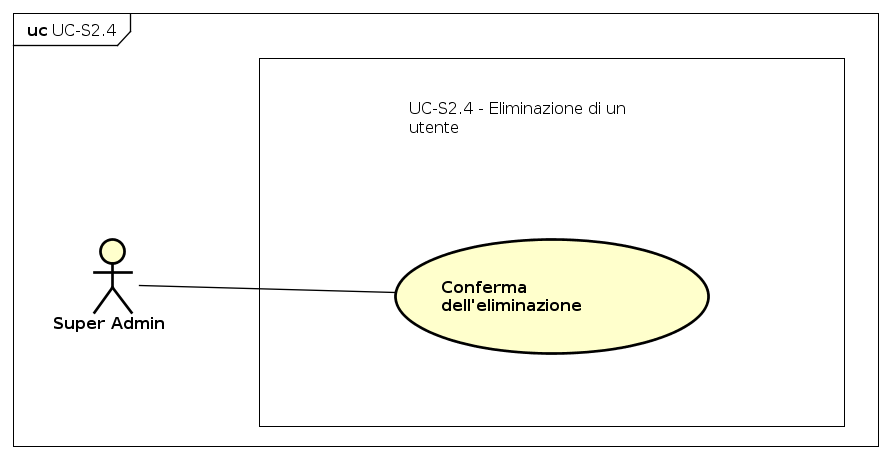
\includegraphics[width=12cm]{res/img/UCSuperadmin/UC-S2.4.png}
%      \caption{UC-S2.4 - Eliminazione di un utente}
%      \end{center} 
%    \end{figure}    
    
    %Tabella 
%    \begin{center}
%     \bgroup
%    \def\arraystretch{1.8}     
%      \begin{longtable}{  p{3.5cm} | p{8cm} } 
        
%        \hline
%        \multicolumn{2}{ | c | }{ \cellcolor[gray]{0.9} \textbf{UC-S2.4 - Eliminazione di un utente }} \\ 
%        \hline
        
%        \textbf{Attori Primari} & \glossaryItem{Super-Admin}\\  
%        \textbf{Scopo e descrizione} & L'\glossaryItem{Attore} entra nella pagina di eliminazione dell'utente, nella quale ha la possibilit\`a
%        di eliminarlo. \\
      
 %       \textbf{Precondizioni}  & L'applicazione richiede la conferma dell'eliminazione dell'utente. \\ 
        
%        \textbf{Postcondizioni} & Il sistema ha seguito le indicazioni dell'\glossaryItem{Attore}. \\ 
%         \textbf{Scenario principale} & 1. L'\glossaryItem{Attore} ha la possibilit\`a di confermare l'eliminazione; 
         
%         2. l'\glossaryItem{Attore} Ha la possibilit\`a ritirare la richiesta di eliminazione. \\
        
%         \textbf{Estensioni} & 1. Uscita dalla pagina senza salvataggio delle modifiche.  \\
     
%     \end{longtable}
%      \egroup
%    \end{center}


\subsubsection{Gestione degli altri Super-Admin}
    \begin{figure}[H]
      \begin{center}
        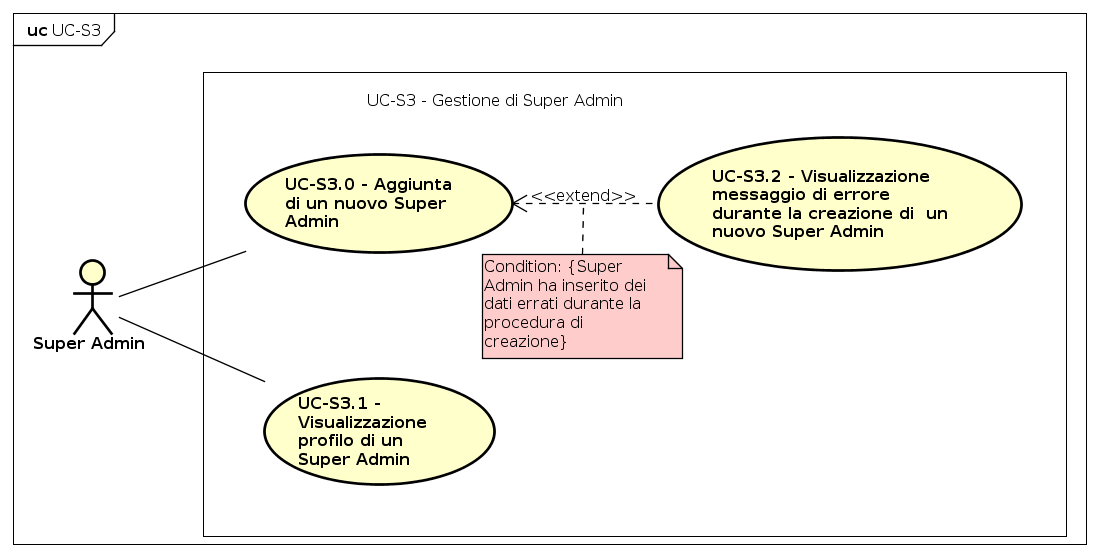
\includegraphics[width=12cm]{res/img/UCSuperadmin/UC-S3.png}
      \caption{UC-S3 - Gestione di altri \glossaryItem{Super-Admin}}
      \end{center} 
    \end{figure}    
    
    %Tabella 
    \begin{center}
      \bgroup
      \def\arraystretch{1.8}     
      \begin{longtable}{  p{3.5cm} | p{8cm} } 
        
        \hline
        \multicolumn{2}{ | c | }{ \cellcolor[gray]{0.9} \textbf{UC-S3 - Gestione degli altri \glossaryItem{Super-Admin} }} \\ 
        \hline
        
        \textbf{Attori Primari} & \glossaryItem{Super-Admin}.\\  
        \textbf{Scopo e descrizione} & Il \glossaryItem{Super-Admin} è entrato nella pagina di gestione dei \glossaryItem{Super-Admin}. In questa pagina può aggiungere un nuovo \glossaryItem{Super-Admin},
vedere in un elenco quelli già presenti e vederne le informazioni in dettaglio cliccando nella voci corrispondenti dell'elenco. \\
        \textbf{Precondizioni}  & Il \glossaryItem{Super-Admin} entra nella pagina di gestione dei \glossaryItem{Super-Admin}.\\ 
        
        \textbf{Postcondizioni} & Il sistema ha preso in carico le indicazioni del \glossaryItem{Super-Admin}. \\ 
         \textbf{Scenario principale} & 1. Il \glossaryItem{Super-Admin} ha la possibilit\`a di aggiungere un nuovo \glossaryItem{Super-Admin}.  (UC-S3.0)
         
         2. Il \glossaryItem{Super-Admin} ha la possibilit\`a di visualizzare in dettaglio il profilo di un \glossaryItem{Super-Admin} esistente. (UC-S3.1) \\
        
         \textbf{Estensioni} & 1. Fallimento dell'inserimento di un \glossaryItem{Super-Admin}. (UC-S3.2) \\
     
     \end{longtable}
      \egroup
    \end{center}


\subsubsection{Creazione di un super-admin}
    \begin{figure}[H]
      \begin{center}
        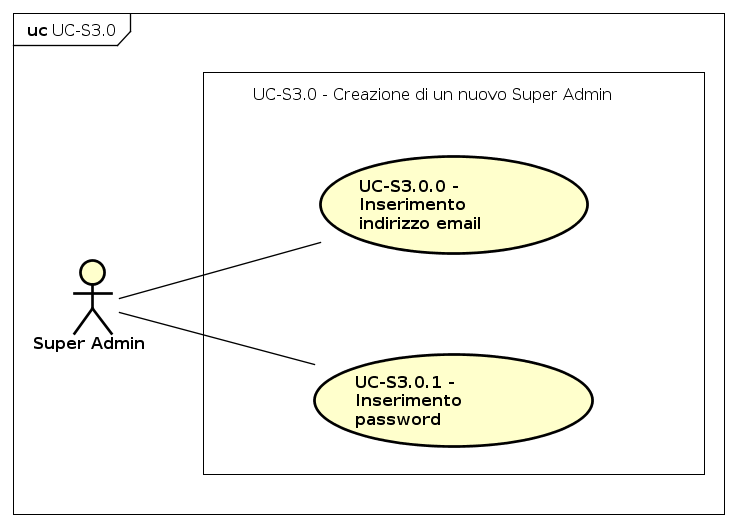
\includegraphics[width=12cm]{res/img/UCSuperadmin/UC-S3.0.png}
      \caption{UC-S3.0 - Creazione di un \glossaryItem{Super-Admin}}
      \end{center} 
    \end{figure}    
    
    %Tabella 
    \begin{center}
      \bgroup
      \def\arraystretch{1.8}     
      \begin{longtable}{  p{3.5cm} | p{8cm} } 
        
        \hline
        \multicolumn{2}{ | c | }{ \cellcolor[gray]{0.9} \textbf{UC-S3.0 - Creazione di un \glossaryItem{Super-Admin} }} \\ 
        \hline
        
        \textbf{Attori Primari} & \glossaryItem{Super-Admin}.\\  
        \textbf{Scopo e descrizione} & Il \glossaryItem{Super-Admin} entra nella pagina di creazione di un altro \glossaryItem{Super-Admin}. 
        Qui deve aggiungere le informazioni (email, password) necessarie per la registrazione di un nuovo \glossaryItem{Super-Admin}. \\
      
        \textbf{Precondizioni}  &  Il \glossaryItem{Super-Admin} entra nella pagina di creazione di un nuovo \glossaryItem{Super-Admin} \\
        \textbf{Postcondizioni} & Il sistema ha creato un nuovo \glossaryItem{Super-Admin} nel database \\ 
         \textbf{Scenario principale} & 1. Il \glossaryItem{Super-Admin} inserisce l'email dell'utente da registrare; (UC-S3.0.0)
         
         2. Il \glossaryItem{Super-Admin} aggiunge una password nell'apposito campo. (UC-S3.0.1)\\
        
     
     \end{longtable}
      \egroup
    \end{center}

    \subsubsection{Inserimento indirizzo email di un nuovo Super-Admin}   
        
        %Tabella 
        \begin{center}
          \bgroup
          \def\arraystretch{1.8}     
          \begin{longtable}{  p{3.5cm} | p{8cm} } 
            
            \hline
            \multicolumn{2}{ | c | }{ \cellcolor[gray]{0.9} \textbf{UC-S3.0.0 - Inserimento indirizzo email}} \\ 
            \hline
            
            \textbf{Attori Primari} & \glossaryItem{Super-Admin} \\ 
            \textbf{Scopo e Descrizione} & Il \glossaryItem{Super-Admin} inserisce l'indirizzo email del nuovo \glossaryItem{Super-Admin} durante la \glossaryItem{procedura} di creazione di un nuovo \glossaryItem{Super-Admin}. \\ 
            
            \textbf{Precondizioni}  & Il \glossaryItem{Super-Admin} ha visualizzato la pagina per la creazione di un nuovo \glossaryItem{Super-Admin}.  \\ 
            
            \textbf{Postcondizioni} & Il campo testo è stato compilato con il contenuto richiesto. \\
             \textbf{Scenario principale} & 1. Il \glossaryItem{Super-Admin} inserisce l'indirizzo email durante la \glossaryItem{procedura} di creazione di un nuovo \glossaryItem{Super-Admin}.\\ 
          \end{longtable}
          \egroup
        \end{center} 
        
    \subsubsection{Inserimento password di un nuovo Super-Admin} 
        
        %Tabella 
        \begin{center}
          \bgroup
          \def\arraystretch{1.8}     
          \begin{longtable}{  p{3.5cm} | p{8cm} } 
            
            \hline
            \multicolumn{2}{ | c | }{ \cellcolor[gray]{0.9} \textbf{UC-S3.0.1 - Inserimento password}} \\ 
            \hline
            
            \textbf{Attori Primari} & \glossaryItem{Super-Admin} \\ 
            \textbf{Scopo e Descrizione} & Il \glossaryItem{Super-Admin} inserisce la password associata all'account del nuovo \glossaryItem{Super-Admin}. \\ 
            
            \textbf{Precondizioni}  & Il \glossaryItem{Super-Admin} ha visualizzato la pagina per la creazione di un nuovo \glossaryItem{Super-Admin}. \\ 
            
            \textbf{Postcondizioni} & Il \glossaryItem{Super-Admin} ha inserito una password associata all'account del nuovo \glossaryItem{Super-Admin}. \\ 
            \textbf{Scenario principale} & 1. Il \glossaryItem{Super-Admin} inserisce una password associata all'account del nuovo \glossaryItem{Super-Admin}.\\
          \end{longtable}
          \egroup
        \end{center}

	\subsubsection{Visualizzazione profilo di un Super-Admin}
	    %Tabella 
	    \begin{center}
	      \bgroup
	      \def\arraystretch{1.8}     
	      \begin{longtable}{  p{3.5cm} | p{8cm} } 
	        
	        \hline
	        \multicolumn{2}{ | c | }{ \cellcolor[gray]{0.9} \textbf{UC-S3.1 - Visualizzazione profilo di un \glossaryItem{Super-Admin} }} \\ 
	        \hline
	        
	        \textbf{Attori Primari} & \glossaryItem{Super-Admin}.\\  
	        \textbf{Scopo e descrizione} & Il \glossaryItem{Super-Admin} è entrato nella pagina di visualizzazione del profilo di un altro \glossaryItem{Super-Admin}. In questa pagina può visualizzare le informazioni del \glossaryItem{Super-Admin} selezionato. \\
	        \textbf{Precondizioni}  & Il \glossaryItem{Super-Admin} ha selezionato un \glossaryItem{Super-Admin}.\\ 
	        
	        \textbf{Postcondizioni} & Il \glossaryItem{Super-Admin} ha visualizzato il profilo del \glossaryItem{Super-Admin} selezionato. \\ 
	         \textbf{Scenario principale} & 1. Il \glossaryItem{Super-Admin} visualizza il profilo del \glossaryItem{Super-Admin} selezionato. \\ 
	     
	     \end{longtable}
	      \egroup
	    \end{center}
	    
	    \subsubsection{Visualizzazione messaggio di errore durante la creazione di un Super-Admin}
	        %Tabella 
	        \begin{center}
	          \bgroup
	          \def\arraystretch{1.8}     
	          \begin{longtable}{  p{3.5cm} | p{8cm} } 
	            
	            \hline
	            \multicolumn{2}{ | c | }{ \cellcolor[gray]{0.9} \textbf{UC-S3.2 - Visualizzazione messaggio di errore nella creazione di un \glossaryItem{Super-Admin} }} \\ 
	            \hline
	            
	            \textbf{Attori Primari} & \glossaryItem{Super-Admin}.\\  
	            \textbf{Scopo e descrizione} & Il \glossaryItem{Super-Admin} ha cercato di inserire un altro \glossaryItem{Super-Admin}, ma si è verificato un errore. \\
	            \textbf{Precondizioni}  & Il \glossaryItem{Super-Admin} ha inserito un indirizzo email duplicato durante la creazione di un altro \glossaryItem{Super-Admin}.\\ 
	            
	            \textbf{Postcondizioni} & Il \glossaryItem{Super-Admin} ha visualizzato un messaggio di errore che lo avvisa dell'inserimento fallito. \\ 
	             \textbf{Scenario principale} & 1. Il \glossaryItem{Super-Admin} visualizza il messaggio di errore dovuto all'inserimento di dati errati durante la creazione di un nuovo \glossaryItem{Super-Admin}. \\ 
	         
	         \end{longtable}
	          \egroup
	        \end{center}

%##################################################################


\newpage
